\apendice{Gráfico de colunas empilhadas}
\label{ap:graphicColBar}

\section{ST-DBSCAN}
\label{ap:stdbscan}

Os resultados exibidos na figura \ref{fig:metricasChi201842501} foram quase nulos devido a baixa quantidade de casos de Chikungunya, e além disso os poucos casos são distantes, logo não atendem ao critério básico de distância máxima entre dois pontos para formar um grupo.
\begin{figure}[!ht]
	\centering	
	\Caption{\label{fig:metricasChi201842501} Métricas ST-DBSCAN: Chikungunya/2018, 4 semanas, Eps = 250, MinPts = 2}
	\UECEfig{}{
		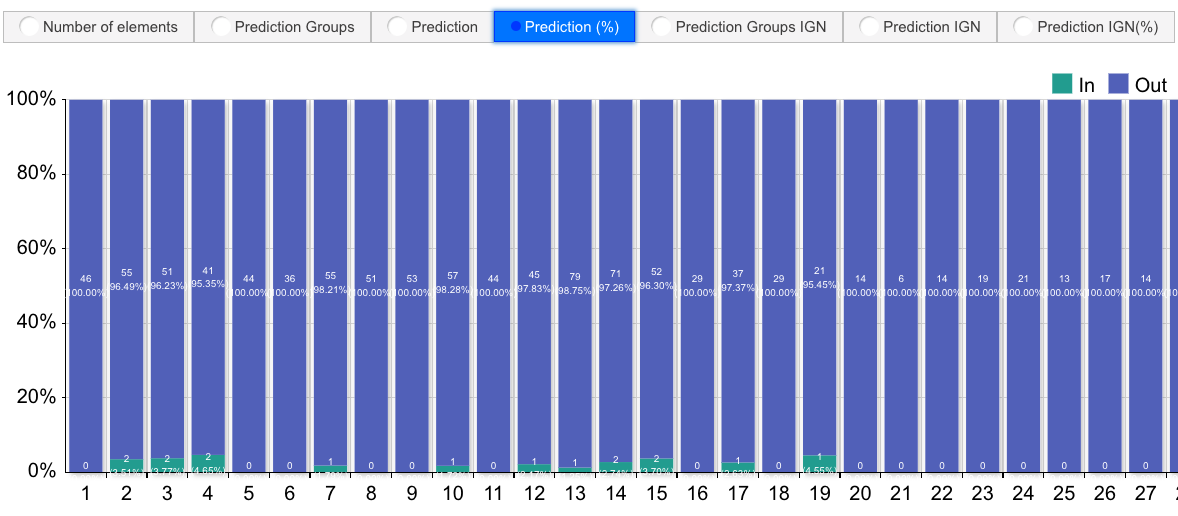
\includegraphics[width=15cm]{figuras/metricas/ST-DBSCAN_2018.png}
	}{
		\Fonte{Elaborado pelo autor}
	}
\end{figure}

\pagebreak
\section{ST-IGN}
\label{ap:stign}

Os resultados em \ref{fig:metricasChi201842501IGN} também foram praticamente nulos devido a baixa quantidade de casos de Chikungunya, e distância máxima entre dois pontos para formar um grupo de 250 metros.
\begin{figure}[!ht]
	\centering	
	\Caption{\label{fig:metricasChi201842501IGN} Métricas ST-IGN: Chikungunya/2018, 4 semanas, Eps = 250, MinPts = 2}
	\UECEfig{}{
		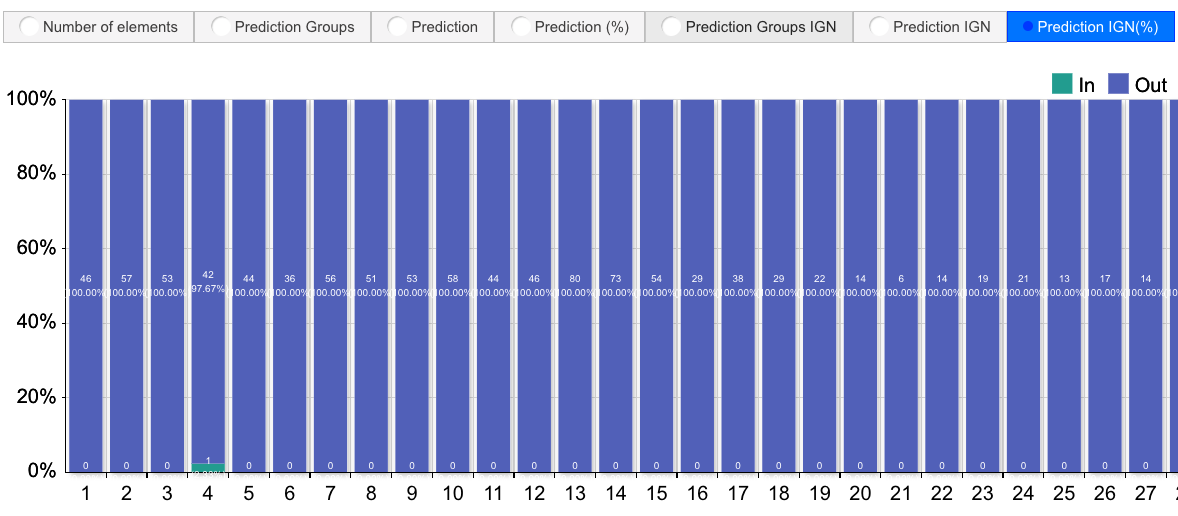
\includegraphics[width=15cm]{figuras/metricas/ST-IGN_2018.png}
	}{
		\Fonte{Elaborado pelo autor}
	}
\end{figure}
\FloatBarrier

\begin{sidewaysfigure}[!ht]
	\centering
	\Caption{\label{fig:metricasDengueBar201745001} Métricas ST-DBSCAN: Dengue/2017, 4 semanas, Eps = 500m, MinPts = 2}
	\UECEfig{}{
		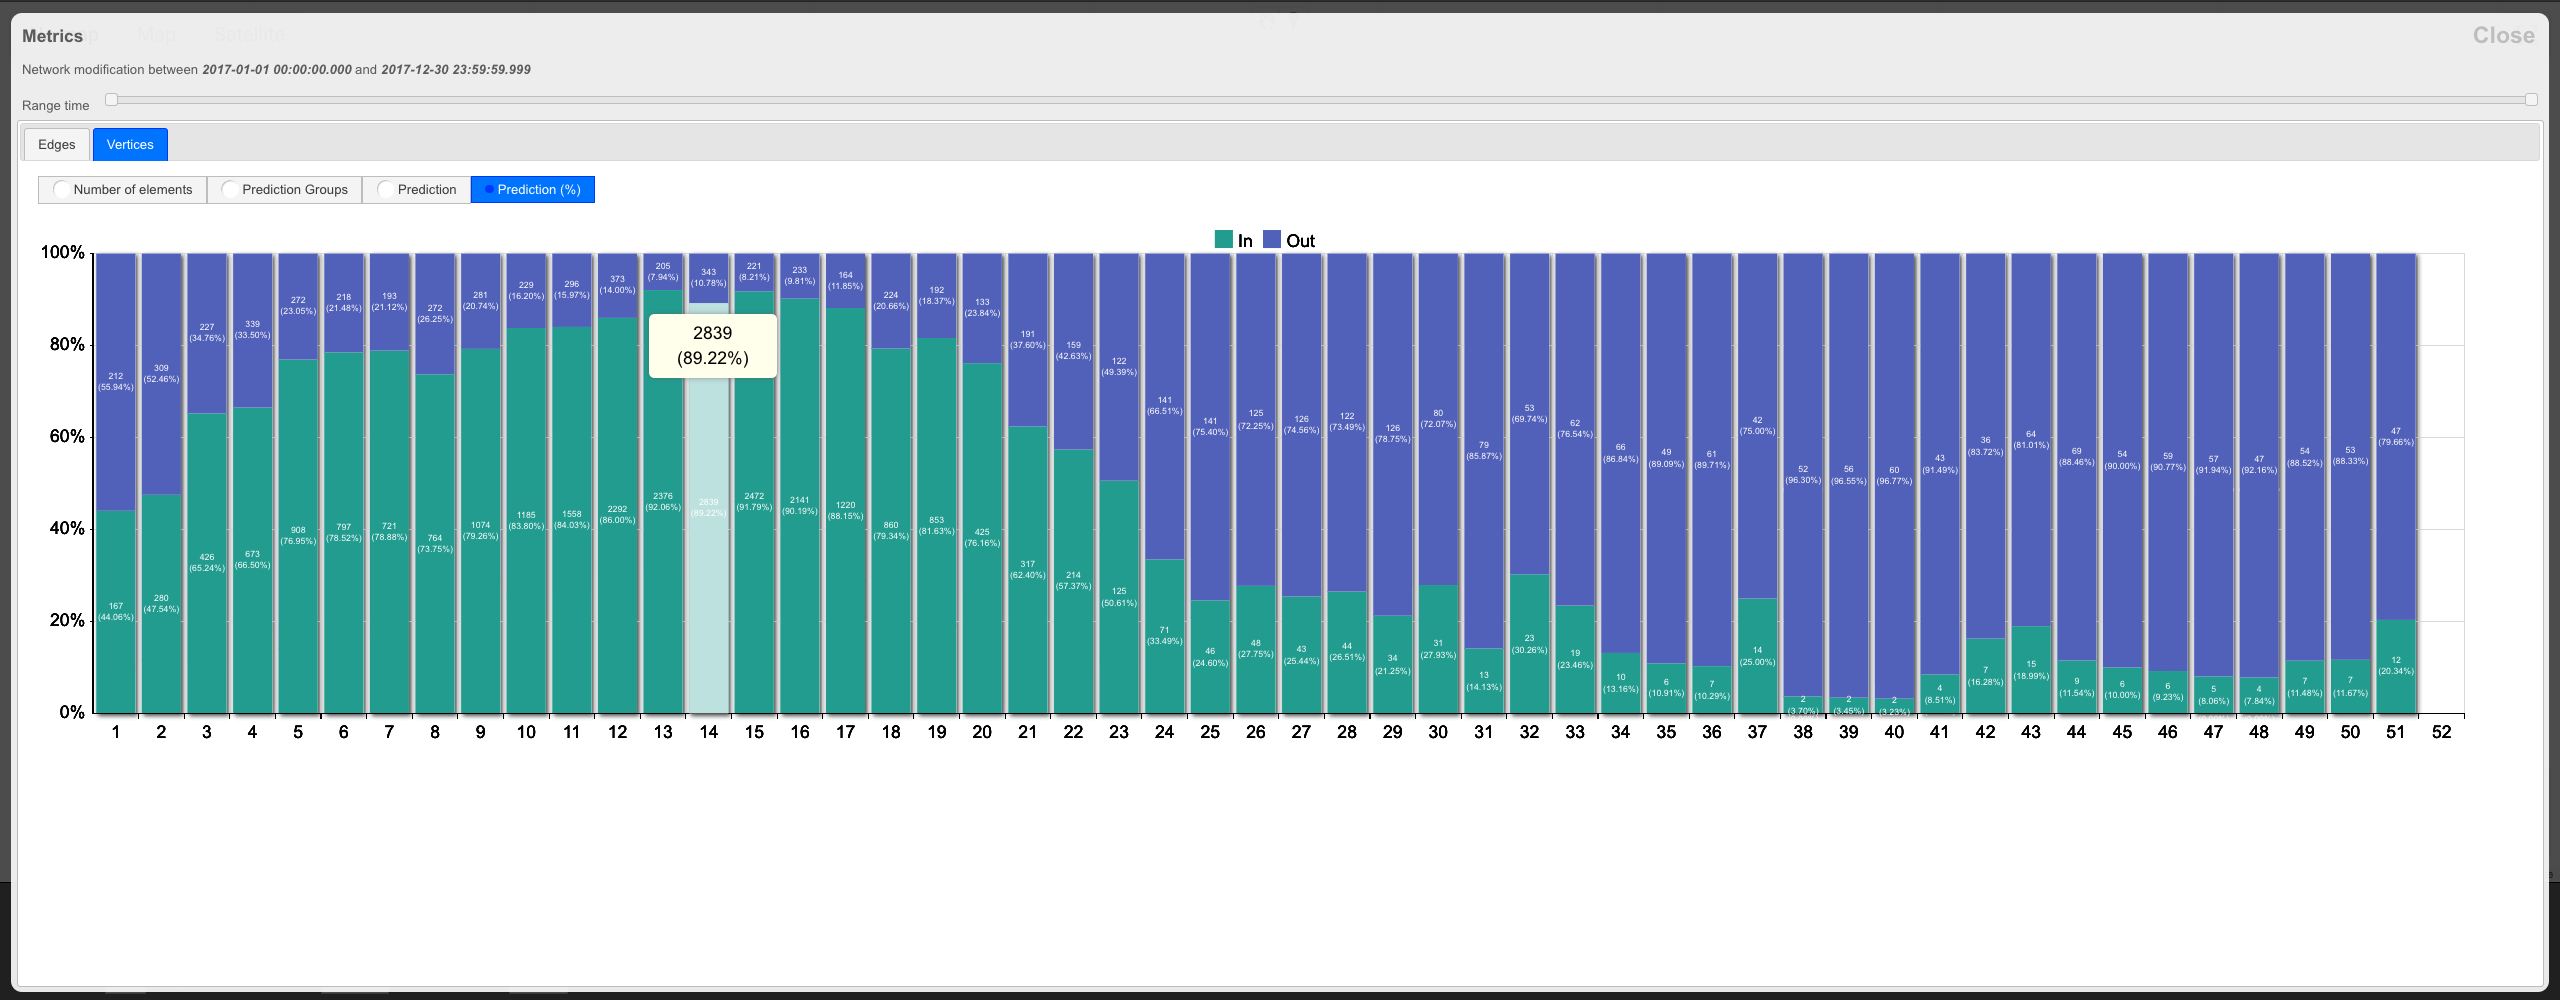
\includegraphics[width=25cm]{figuras/metricas/dengue2017chartbar.png}
	}{
		\Fonte{Elaborado pelo autor}
	}
\end{sidewaysfigure}


\begin{sidewaysfigure}[!ht]
	\centering	
	\Caption{\label{fig:metricasDengueBar201845001} Métricas ST-DBSCAN: Dengue/2018, 4 semanas, Eps = 500m, MinPts = 2}
	\UECEfig{}{
		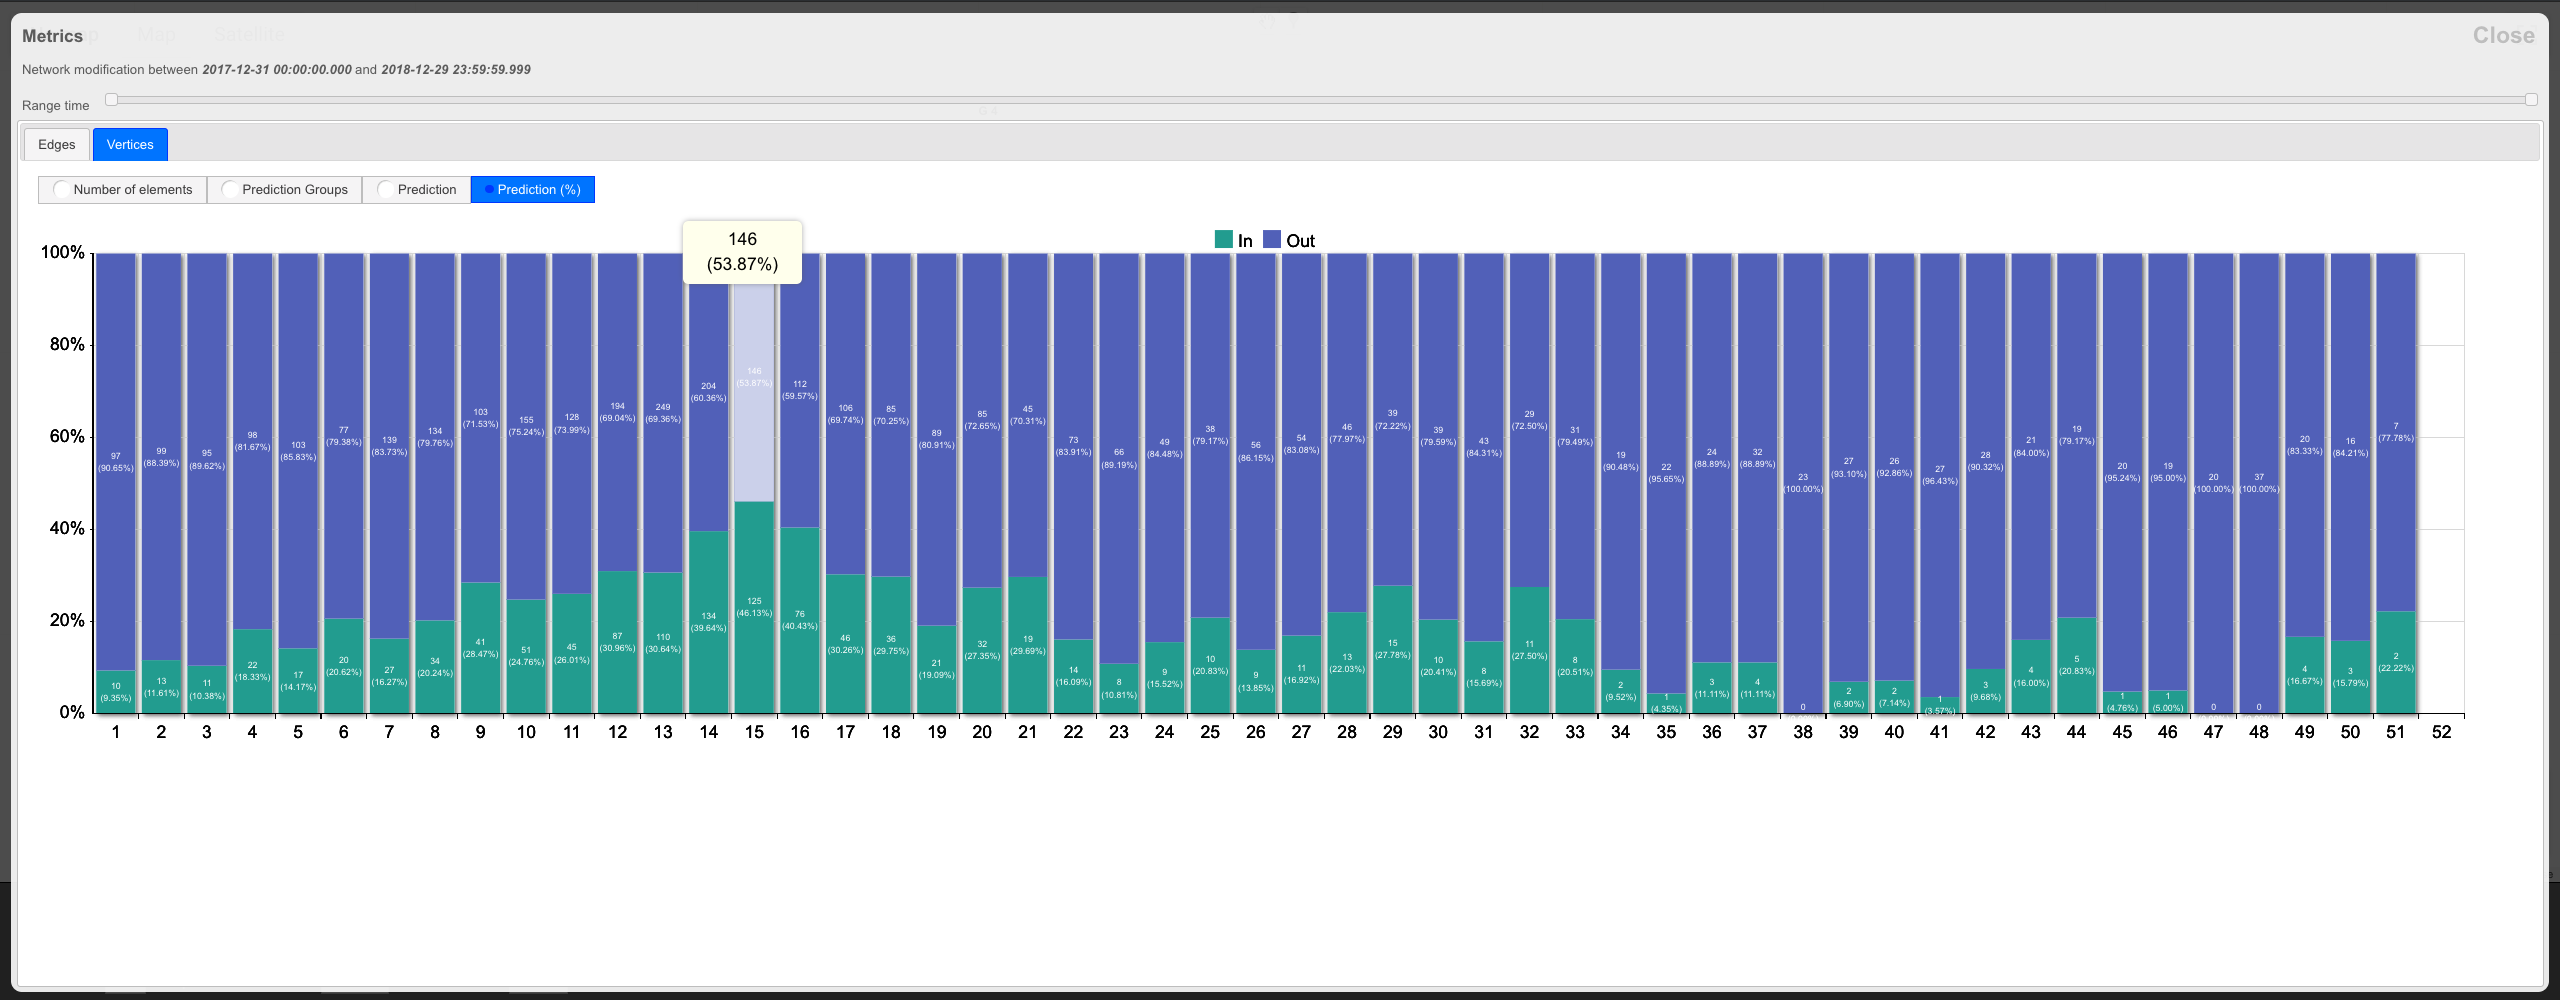
\includegraphics[width=25cm]{figuras/metricas/dengue2018chartbar.png}
	}{
		\Fonte{Elaborado pelo autor}
	}
\end{sidewaysfigure}


\begin{sidewaysfigure}[!ht]
	\centering	
	\Caption{\label{fig:metricasChi201745002} Métricas ST-DBSCAN: Chikungunya/2017, 4 semanas, Eps = 500m, MinPts = 2}
	\UECEfig{}{
		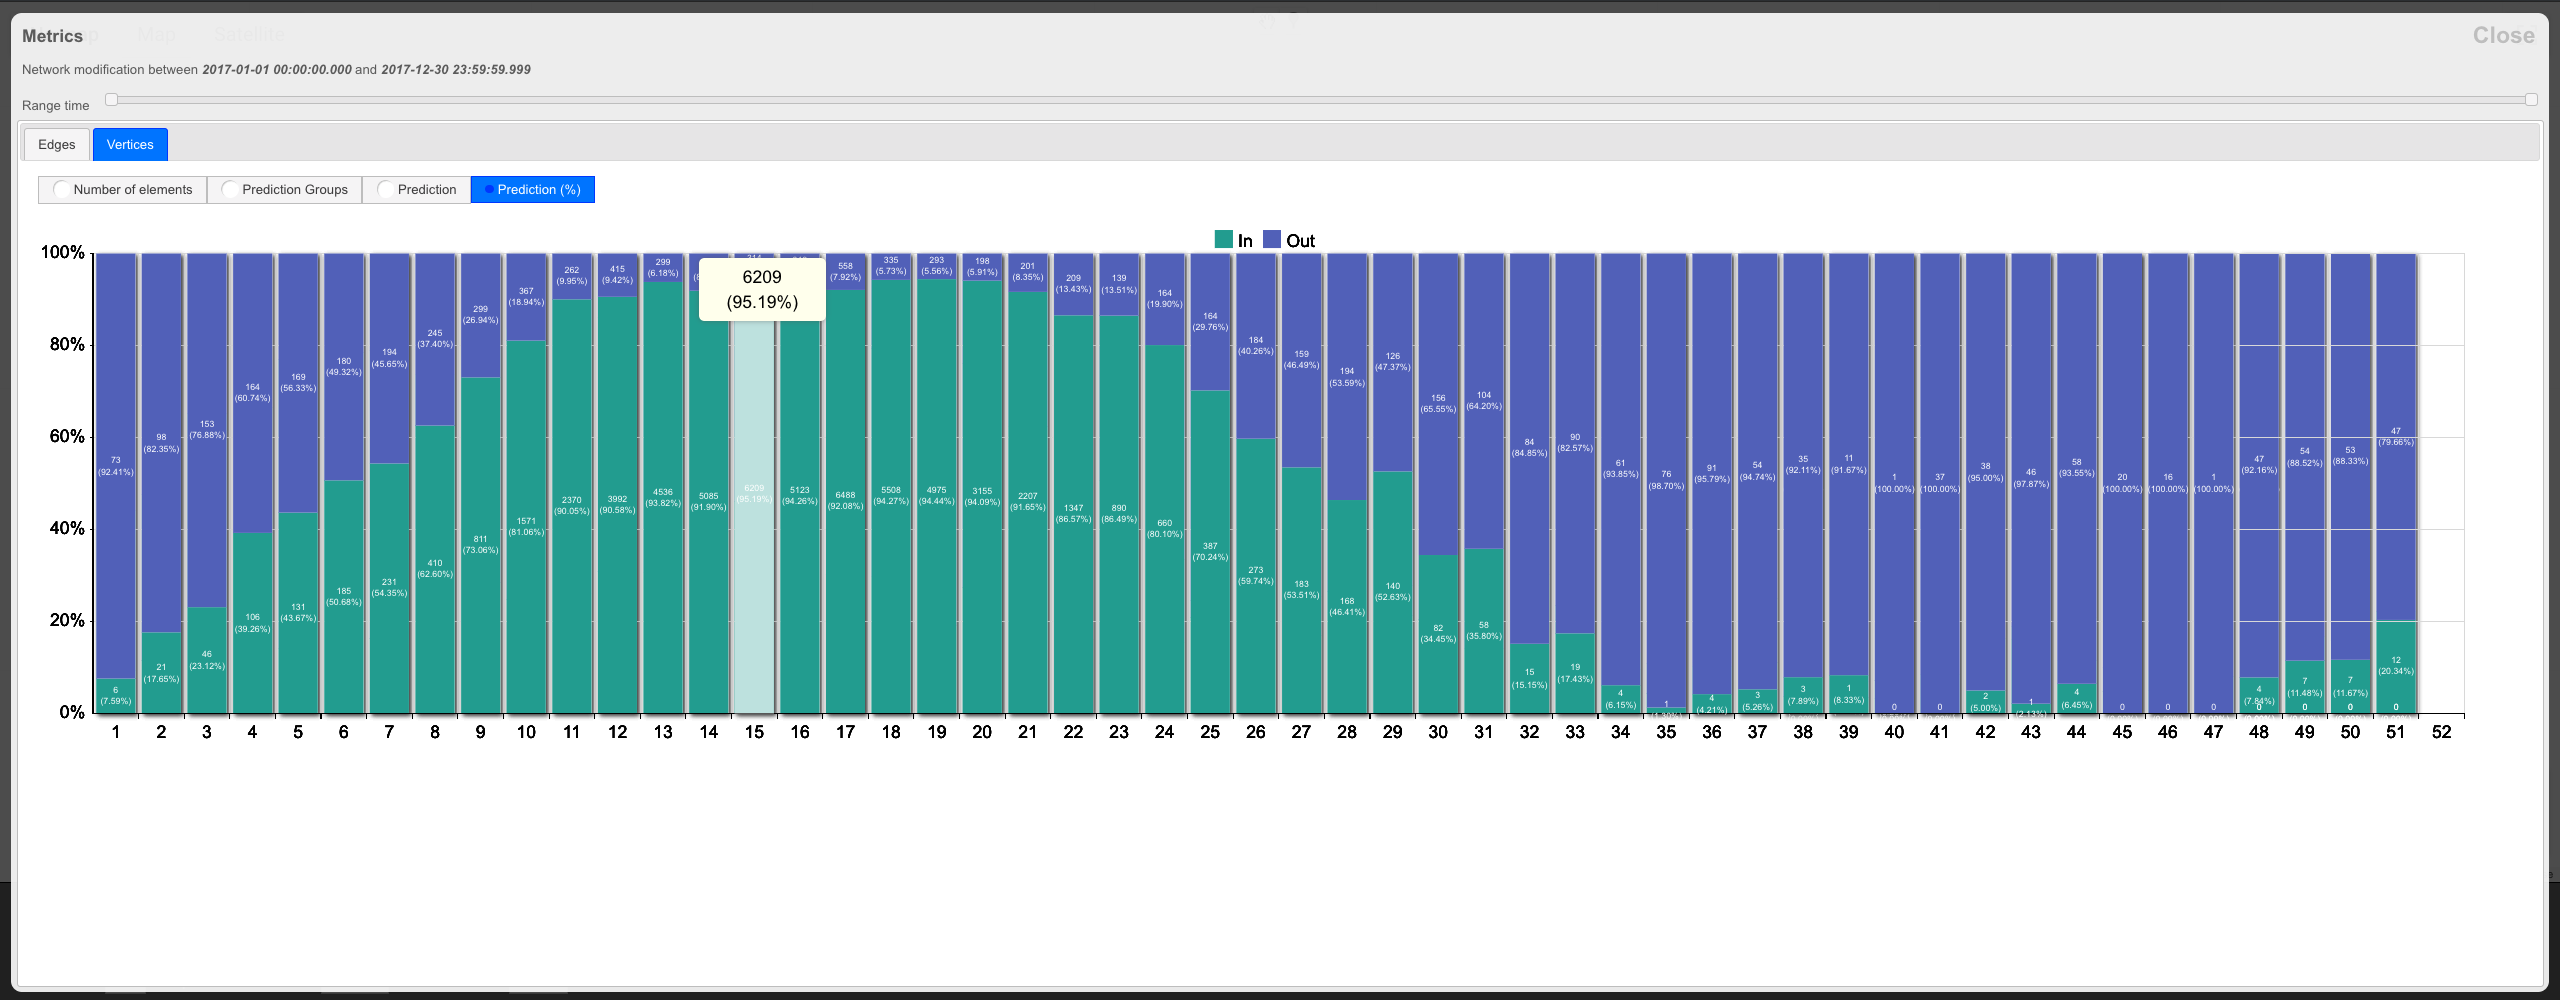
\includegraphics[width=25cm]{figuras/metricas/chikungunya2017chartbar.png}
	}{
		\Fonte{Elaborado pelo autor}
	}
\end{sidewaysfigure}


\begin{sidewaysfigure}[!ht]
	\centering
	\Caption{Métricas ST-IGN: Chikungunya/2017, 4 semanas, Eps = 250, MinPts = 2}
	\UECEfig{}{
		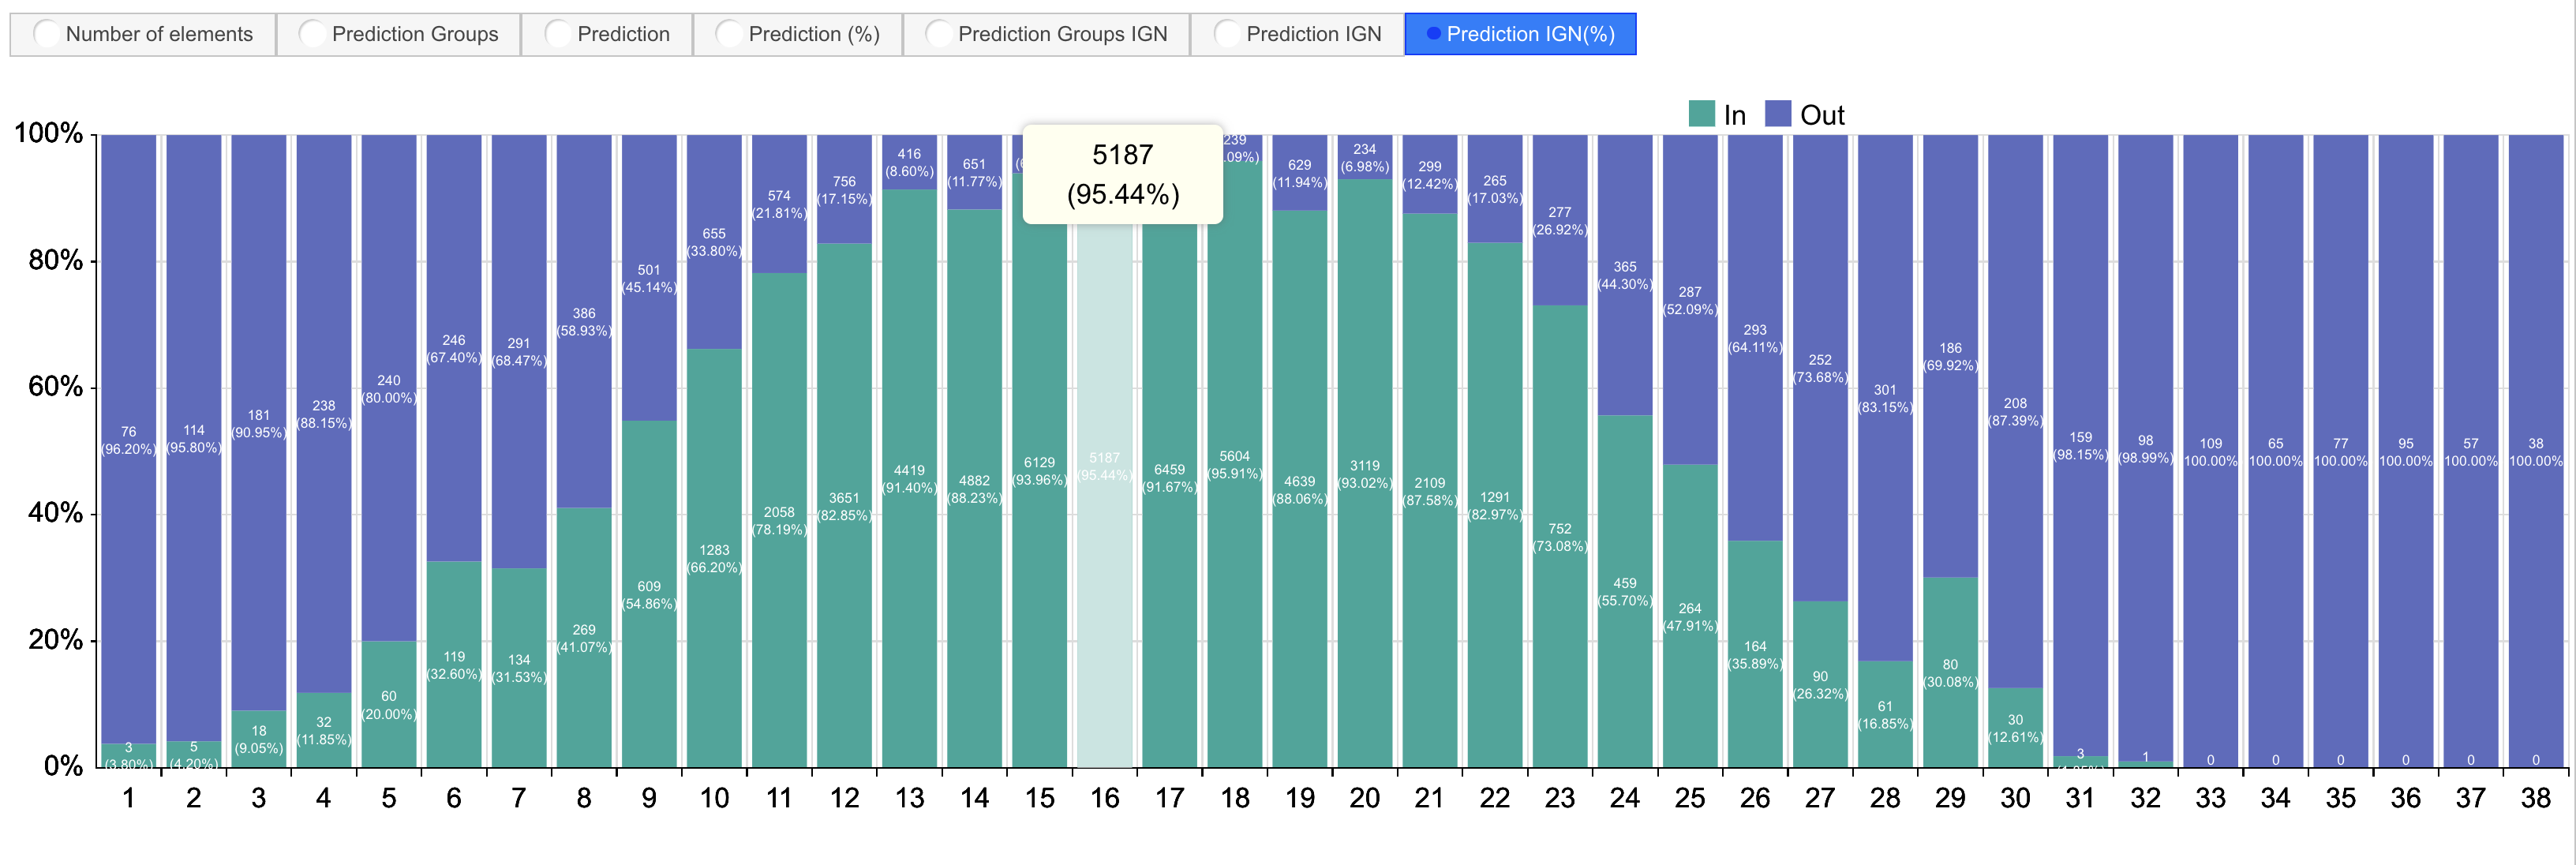
\includegraphics[width=25cm]{figuras/predicao/2017/Pred_ST-IGN_Chikungunya_2017_percent.png}
	}{
		\Fonte{Elaborado pelo autor}
	}
\end{sidewaysfigure}

\begin{sidewaysfigure}[!ht]
	\centering
	\Caption{Métricas ST-IGN: Dengue/2017, 4 semanas, Eps = 250, MinPts = 2}
	\UECEfig{}{
		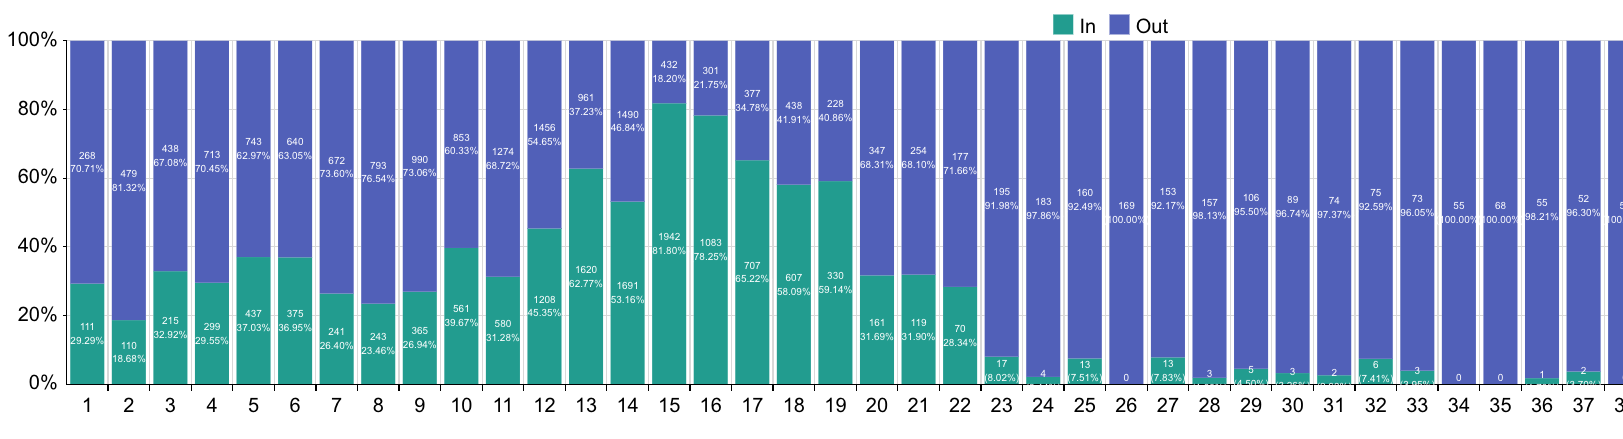
\includegraphics[width=25cm]{figuras/predicao/2017/Pred_ST-IGN_Dengue_2017_percent.png}
	}{
		\Fonte{Elaborado pelo autor}
	}
\end{sidewaysfigure}

\begin{sidewaysfigure}[!ht]
	\centering
	\Caption{Métricas ST-IGN: Dengue/2018, 4 semanas, Eps = 250, MinPts = 2}
	\UECEfig{}{
		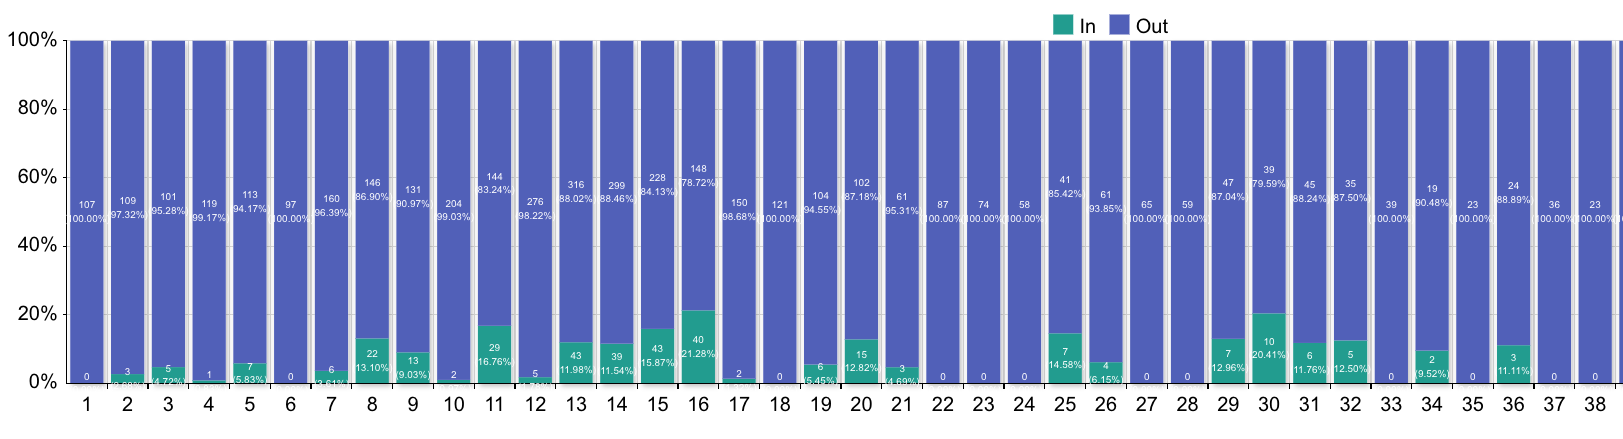
\includegraphics[width=25cm]{figuras/predicao/2018/Pred_ST-IGN_Dengue_2018_percent.png}
	}{
		\Fonte{Elaborado pelo autor}
	}
\end{sidewaysfigure}
